\documentclass[11pt]{article}

\usepackage{fancybox}



\usepackage{color}
\usepackage{url}
\usepackage[margin=1in]{geometry}


\renewcommand{\textfraction}{0.0}
\renewcommand{\topfraction}{1.0}
%\renewcommand{\textfloatsep}{5mm}

\usepackage{comment}
% Definitions of handy macros can go here
\usepackage{amsmath,amssymb,amsthm,bm,mathtools}
\usepackage{multirow}
%\usepackage{dsfont,multirow,hyperref,setspace,natbib,enumerate}
\usepackage{dsfont,multirow,hyperref,setspace,enumerate}
\hypersetup{colorlinks,linkcolor={blue},citecolor={blue},urlcolor={red}} 
\usepackage{algpseudocode,algorithm}
\algnewcommand\algorithmicinput{\textbf{Input:}}
\algnewcommand\algorithmicoutput{\textbf{Output:}}
\algnewcommand\INPUT{\item[\algorithmicinput]}
\algnewcommand\OUTPUT{\item[\algorithmicoutput]}

\mathtoolsset{showonlyrefs=true}



\theoremstyle{plain}
\newtheorem{thm}{Theorem}[section]
\newtheorem{lem}{Lemma}
\newtheorem{prop}{Proposition}
\newtheorem{pro}{Property}
\newtheorem{assumption}{Assumption}

\theoremstyle{definition}
\newtheorem{defn}{Definition}
\newtheorem{cor}{Corollary}
\newtheorem{example}{Example}
\newtheorem{rmk}{Remark}


\renewcommand{\thefigure}{{S\arabic{figure}}}%
\renewcommand{\thetable}{{S\arabic{table}}}%
\renewcommand{\figurename}{{Supplementary Figure}}    
\renewcommand{\tablename}{{Supplementary Table}}    
\setcounter{figure}{0}   
\setcounter{table}{0}  


\def\MLET{\hat \Theta_{\text{MLE}}}
\newcommand{\cmt}[1]{{\leavevmode\color{red}{#1}}}



\usepackage{dsfont}

\usepackage{multirow}

\DeclareMathOperator*{\minimize}{minimize}



\usepackage{mathtools}
\mathtoolsset{showonlyrefs}
\newcommand*{\KeepStyleUnderBrace}[1]{%f
  \mathop{%
    \mathchoice
    {\underbrace{\displaystyle#1}}%
    {\underbrace{\textstyle#1}}%
    {\underbrace{\scriptstyle#1}}%
    {\underbrace{\scriptscriptstyle#1}}%
  }\limits
}
\usepackage{xr}
\externaldocument{tensor_regression_nips_clean}
\input macros.tex





\title{Supplements for ``Exponential tensor regression with covariates on multiple modes''}


\begin{document}


\begin{center}
\begin{spacing}{1.5}
\textbf{\Large Supplements for ``Exponential tensor regression with \\
covariates on multiple modes''}
\end{spacing}
\end{center}

\section{Proofs}
\begin{proof}[Proof of Theorem~\ref{thm:main}]
Define $\ell(\tB)=\mathbb{E}(\tL_{\tY}(\tB))$, where the expectation is taken with respect to $\tY\sim \trueB$ under the model with true parameter $\trueB$. We first prove the following two conclusions:
\begin{enumerate}
\item[C1.] There exists two positive constants $C_1$, $C_2>0$, such that, with probability at least $1-\exp(-C_1\log K\sum_k p_k)$, the stochastic deviation, $\tL_{\tY}(\tB)-\ell(\tB)$, satisfies
\[
|\tL_{\tY}(\tB)-\ell(\tB)|=|\langle \tE,\ \tB\times_1\mX_1\times_2\cdots\times_K \mX_K\rangle| \leq C_2\FnormSize{}{\tB} \log K\sqrt{{\prod_k r_k \over \max_k r_k} \sum_k p_k}.
\]
\item[C2.] The inequality $\ell(\hat \tB) - \ell(\trueB) \leq  -{L\over 2}\FnormSize{}{\hat \Theta-\trueT}^2$ holds, where $L>0$ is the lower bound for $\min_{|\theta|\leq \alpha}|b''(\theta)|$. 
\end{enumerate}

To prove C1, we note that the stochastic deviation can be written as:
\begin{align}\label{bound}
\tL_{\tY}(\tB)-\ell(\tB)&=\langle \tY-\mathbb{E}(\tY|\tX),\ \Theta(\tB)\rangle\notag \\
&= \langle \tY- b'(\trueT),\ \Theta\rangle \notag \\
&= \langle \tE\times_1\mX^T_1\times_2\cdots\times_K\mX^T_K,\ \tB\rangle,
\end{align}
where $\tE=\entry{\varepsilon_{i_1,\ldots,i_K}}\stackrel{\text{def}}{=}\tY-b'(\trueT)$. Based on Proposition~\ref{prop}, $\varepsilon_{i_1,\ldots,i_K}$ is sub-Gaussian-$(\phi U)$. Let $\check\tE\stackrel{\text{def}}{=}\tE\times_1\mX^T_1\times_2\cdots\times_K\mX^T_K$. By the property of sub-Gaussian r.v's, $\check \tE$ is a $(p_1,\ldots,p_K)$-dimensional sub-Gaussian tensor with parameter bounded by $C_2=\phi Uc^{K}_2$. Here $c_2>0$ is the upper bound of $\sigma_{\max}(\mX_k)$. Applying Cauchy-Schwarz inequality to~\eqref{bound} yields
\begin{equation}\label{eq:bound2}
|\tL_{\tY}(\tB)-\ell(\tB)|\leq \norm{\check \tE} \nnorm{\tB},
\end{equation}
where $\norm{\cdot}$ denotes the tensor spectral norm and $\nnorm{\cdot}$ denotes the tensor nuclear norm. The nuclear norm $\nnorm{\tB}$ is  bounded by $\nnorm{\tB}\leq \sqrt{{\prod_k r_k \over \max_k r_k}}\FnormSize{}{\tB}$ (c.f.~\cite{wang2018learning,wang2017operator}). The spectral norm $\norm{\check \tE}$ is bounded by $\norm{\check \tE}\leq C_1 Uc^{K} \log K \sqrt{\sum_k p_k}$ with probability at least $1-\exp(-C_2\log K \sum_kp_k)$ (c.f.~\cite{wang2018learning,tomioka2014spectral}). Combining these two bounds with~\eqref{eq:bound2}, we have, with probability at least $1-\exp(-C_2\log K \sum_kp_k)$, 
\[
|\tL_{\tY}(\tB)-\ell(\tB)|\leq C_1Uc_2^{K}\FnormSize{}{\tB} \log K  \sqrt{ {\prod_k r_k\over \max_k r_k}\sum_k p_k}.
\]

Next we prove C2. Applying Taylor expansion to $\ell(\tB)$ around $\trueB$, 
\begin{equation}\label{eq:log}
\ell(\tB)=\ell(\trueB)+{1\over 2}\text{vec}(\tB-\trueB)^T \tH_{\tY}(\check \tB)\text{vec}(\tB-\trueB),
\end{equation}
where $\tH_{\tY}(\check \tB)$ is the (non-random) Hession of ${\partial \ell^2 (\tB)\over\partial^2 \tB}$ evaluated at $\check \tB =\alpha \text{vec}(\alpha \tB+(1-\alpha)\trueB)$ for some $\alpha\in[0,1]$. Recall that $b''(\theta)=\text{Var}(y|\theta)$, because $y\in\mathbb{R}$ follows the exponential family distribution with function $b(\cdot)$. By chain rule and the fact that $\Theta=\Theta(\tB)=\tB\times_1\mX_1\cdots\times_K\mX_K$, the equation~\eqref{eq:log} implies that
\begin{equation}\label{eq:log2}
\ell(\tB)-\ell(\trueB)=-{1\over 2}\sum_{i_1,\ldots,i_K}b''(\check \theta_{i_1,\ldots,i_K}) (\theta_{i_1,\ldots,i_K}-\theta_{\text{true},i_1,\ldots,i_K})^2 \leq -{L \over 2}\FnormSize{}{\Theta-\trueT}^2,
\end{equation}
holds for all $\tB\in\tP$, provided that $\min_{|\theta|\leq \alpha}|b''(\theta)|\geq L>0$. In particular, the inequality~\eqref{eq:log2} also applies to the constrained MLE $\hat \tB$. So we have
\begin{equation}\label{upperbound}
\ell(\hat \tB)-\ell(\trueB)\leq -{L \over 2}\FnormSize{}{\hat \Theta-\trueT}^2.
\end{equation}
Now we have proved both C1 and C2. Note that $\tL_{\tY}(\hat \tB)- \tL_{\tY}(\trueB)\geq 0$ by the definition of $\hat \tB$, This implies that
\begin{align}
0&\leq \tL_{\tY}(\hat \tB)- \tL_{\tY}(\trueB) \\
&\leq \left(\tL_{\tY}(\hat \tB)-\ell(\hat \tB)\right)-\left( \tL_{\tY}(\trueB)-\ell(\trueB)\right)+\left(\ell(\hat \tB)-\ell(\trueB)\right)\\
&\leq \langle\tE,\ \Theta-\trueT    \rangle -{L\over 2}\FnormSize{}{\hat \Theta-\trueT}^2,
%&\leq 2\sup_{\tB}|\tL_{\tY}(\tB)-\ell(\tB)|-{L\over 2}\FnormSize{}{\hat \Theta-\trueT}^2
\end{align}
where the second line follows from~\eqref{upperbound}. Therefore,
\begin{align}\label{eq:1}
\FnormSize{}{\hat \Theta-\trueT}&\leq {2\over L}\big\langle \tE,\ {\hat \Theta -\trueT \over \FnormSize{}{\hat \Theta-\trueT}} \big\rangle\notag \\
&\leq {2\over L}\sup_{\Theta: \FnormSize{}{\Theta}=1, \Theta=\tB\times_1\mX_1\times_2\cdots\times_K \mX_K}\langle \tE,\ \Theta \rangle\notag \\
&\leq {2\over L}\sup_{\tB\in\tP: \FnormSize{}{\tB}\leq \prod_k \sigma^{-1}_{\min}(\mX_k)} \langle \tE,\ \ \tB\times_1\mX_1\times_2\cdots\times_K\mX_K\rangle.
\end{align}
Combining~\eqref{eq:1} with C1 yields the desired conclusion. 

%\[
%\FnormSize{}{\hat \Theta-\trueT}\leq {2R\over L}  \sum_{i=1} p_i ()
%\]
%\[
%\FnormSize{}{\hat \Theta-\trueT}^2\leq {2\over L}\sup_{\tB: \FnormSize{}{\tB}=1}|\tL_{\tY}(\tB)-\ell(\tB)|\leq {2\over L} \sum_k p_k
%\]
%holds with probability at least $1-\exp(C_1\sum_k p_k)$.
\end{proof}

\begin{prop}[sub-Gaussian residual]\label{prop}
Define the residual tensor $\tE=\entry{\varepsilon_{i_1,\ldots,i_K}}=\tY-b'(\Theta)\in\mathbb{R}^{d_1\times \cdots \times d_K}$. Under the Assumption A2, $\varepsilon_{i_1,\ldots,i_K}$ is a sub-Gaussian random variable with sub-Gaussian parameter bounded by $\phi U$, for all $(i_1,\ldots,i_K)\in[d_1]\times\cdots\times[d_K]$.
\end{prop}
\begin{proof} The proof is similar to Lemma 3 in~\cite{fan2019generalized}. For ease of presentation, we drop the subscript $(i_1,\ldots,i_K)$ and simply write $\varepsilon$ ($=y-b'(\theta)$). For any given $t\in\mathbb{R}$, we have
\begin{align}
\mathbb{E}(\exp(t\varepsilon|\theta)&=\int c(x) \exp\left({\theta x - b(\theta)\over \phi}   \right)\exp \left(t(x-b'(\theta))\right)dx\\
&=\int c(x)\exp \left( {(\theta + \phi t)x - b (\theta+\phi t)+b(\theta+\phi t)-b(\theta)-\phi t b'(\theta) \over \phi}\right)dx\\
&=\exp\left( {b(\theta+\phi t)-b(\theta)-\phi t b'(\theta) \over \phi} \right)\\
&\leq \exp\left(\phi U t^2\over 2 \right),
\end{align}
where $c(\cdot)$ and $b(\cdot)$ are known functions in the exponential family corresponding to $y$. 
Therefore, $\varepsilon$ is sub-Gaussian-$(\phi U)$. 
\end{proof}

\begin{proof}[Proof of Theorem~\ref{thm:KL}]
The proof is similar to~\cite{baldin2018optimal}. We sketch the main steps here for completeness. Recall that $\ell(\tB)=\mathbb{E}(\tL_{\tY}(\tB))$. By the definition of KL divergence, we have that,
\begin{align}
\ell(\hat \tB)&=\ell(\trueB)-\sum_{(i_1,\ldots,i_K)} KL(\theta_{\text{true}, i_1,\ldots, i_K}, \hat \theta_{i_1,\ldots,i_K})\\
&=\ell(\trueB)-\text{KL}(\mathbb{P}_{\tY_{\text{true}}},\ \mathbb{P}_{\hat \tY}),
\end{align}
where $\mathbb{P}_{\tY_{\text{true}}}$ denotes the distribution of $\tY|\tX$ with true parameter $\trueB$, and $\mathbb{P}_{\hat \tY}$ denotes the distribution with estimated parameter $\hat \tB$. Therefore
\begin{align}
\text{KL}(\mathbb{P}_{\tY_{\text{true}}},\ \mathbb{P}_{\hat \tY}) &= \ell(\trueB)-\ell(\hat \tB)\\
&={1\over 2}\sum_{i_1\ldots,i_K}b''(\check \theta_{i_1,\ldots,i_K})(\theta_{i_1,\ldots,i_K}-\theta_{\text{true},i_1,\ldots,i_K})^2\\
&\leq {U\over 2} \FnormSize{}{\Theta-\trueT}^2\\
&\leq {U \over 2}c^{2K}_2\FnormSize{}{\tB-\trueB}^2,
\end{align}
where the second line comes from~\eqref{eq:log}, and $c_2>0$ is the upper bound for the $\sigma_{\max}(\mX_k)$. The result then follows from Theorem~\ref{thm:main}.
\end{proof}

\section{Numerical implementation}
\subsection{Algorithm}
Here we provide the detailed alternating algorithm.
\begin{figure*}[hb]
  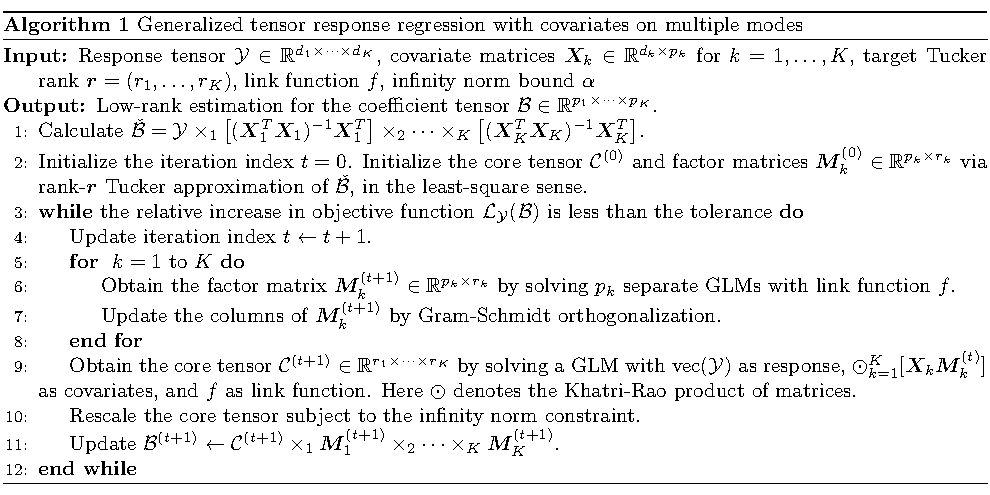
\includegraphics[width=16cm]{algorithm.pdf}
\end{figure*}

\subsection{Time complexity}
The computational complexity of our tensor regression model is $O(d)$ for each loop of iterations, where $d=\prod_k d_k$ is the total size of the response tensor. More precisely, the update of core tensor costs $O(r^3d)$, where $r=\sum_k r_k$ is the total size of the core tensor. The update of one factor matrix $\mM_k$ costs $O(dp_k^3r_k^3)$. Therefore the cost for updating $K$ factors in total is $O( \sum_k dp_k^3r_k^3)\approx  O(d)$

\begin{comment}
The computational complexity of our tensor regression model is $O(d^3+d)$ for each loop of iterations, where $d=\prod_k d_k$ is the total size of the response tensor. More precisely, the update of core tensor costs $O(r^3d^3)$, where $r=\sum_k r_k$ is the total size of the core tensor. The update of factor matrix $\mM_k$ involves solving $p_k$ separate GLMs. Solving those GLMs requires $O(r_k^3 p_k + p_kr_k^3 dd^{-1}_k)$, and therefore the cost for updating $K$ factors in total is $O( \sum_k r^3_k p_k d_k + d\sum_k r_k^3 p_k d_k^{-1})\approx O(\sum p_k d_k +d)\approx O(d)$. 
\end{comment}

\section{Additional results for simulation}
Here we provide the experiment results for assessing our BIC criterion~\eqref{eq:BIC}. We consider the balanced situation where $d_k=d$, $p_k=0.4d_k$ for $k=1,2,3$. We set $\alpha=10$ and consider various combinations of dimension $d$ and rank $\mr=(r_1,r_2,r_3)$. For each combination, we simulate tensor data following Gaussian, Bernoulli, and Poisson models. We then minimize BIC using a grid search over three dimensions. The hyper-parameter $\alpha$ is set to infinity in the fitting, which essentially imposes no prior on the coefficient magnitude. Table~\ref{tab:rank} reports the selected rank averaged over $n_{\text{sim}}=30$ replicates for Gaussian and Poisson models. We found that when $d=20$, the selected rank is slightly smaller than the true rank, and the accuracy improves immediately when the dimension increases to $d=40$. This agrees with our expectation, as in tensor regression, the sample size is related to the number of entries. A larger $d$ implies a larger sample size, so the BIC selection becomes more accurate. 

\begin{table}[ht]
\centering
\resizebox{.8\textwidth}{!}{
\begin{tabular}{|c|cc|cc|}
\hline
True Rank &\multicolumn{2}{c|}{Dimension (Gaussian tensors)}&\multicolumn{2}{c|}{Dimension (Poisson tensors)}\\
$\mr$& $d=20$  &$d=40$&$d=20$ &$d=40$\\
\hline
$(3,\ 3,\ 3)$&$(2.1,\ 2.0,\ 2.0)$&$({\bf 3},\ {\bf 3},\ {\bf 3})$&$(2.0,\ 2.2,\ 2.1)$&$({\bf 3},\ {\bf 3},\ {\bf 3})$\\
$(4,\ 4,\ 6)$&$(3.2,\ 3.1,\ 5.0)$&$({\bf 4},\ {\bf 4},\ {\bf 6})$&$({\bf 4.0},\ {\bf 4.0},\ 5.2)$&$({\bf 4},\ {\bf 4},\ {\bf 6})$\\
$(6,\ 8,\ 8)$&$(5.1,\ 7.0,\ 6.9)$&$({\bf 6},\ {\bf 8},\ {\bf 8})$&$(5.0,\ 6.1,\ 7.1)$&$({\bf 6},\ {\bf 8},\ {\bf 8})$\\
\hline
\end{tabular}
}
\vspace{.2cm}
\caption{Rank selection via BIC. Bold number indicates no significant difference between the estimate and the ground truth, based on a $z$-test with a level 0.05.}\label{tab:rank}
\vspace{-.4cm}
\end{table}

\section{Additional results for real data analysis}
Here we provide additional results for the real data analysis. 


\subsection{HCP data analysis}


Supplement Figure~\ref{fig:s1} compares the estimated coefficients from our method (tensor regression) with those from classical GLM approach. A classical GLM is to regress the brain edges, one at a time, on the individual-level covariates, and this logistic model is repeatedly fitted for every edge $\in [68]\times [68]$. As we can see in the figure, our tensor regression shrinkages the coefficients towards center, thereby enforcing the sharing between coefficient entries. 

\begin{figure}[ht]
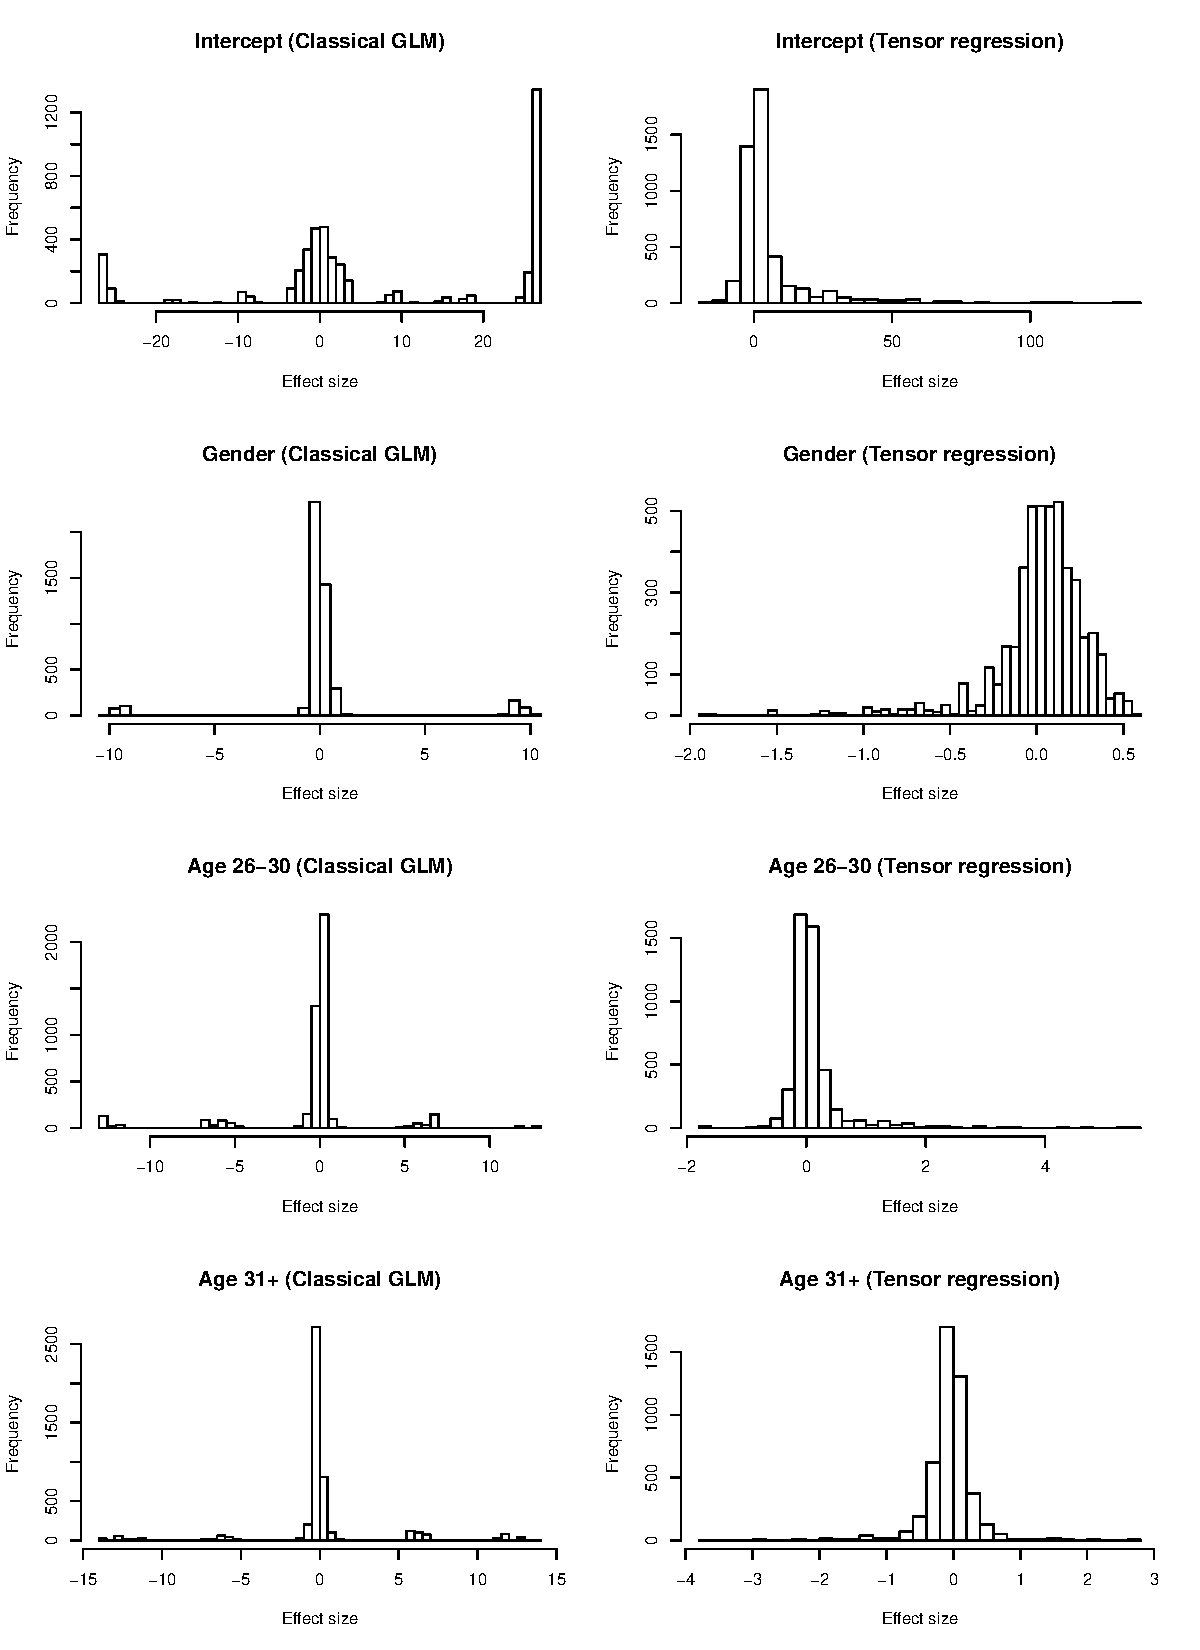
\includegraphics[width=17cm]{compare.pdf}
\caption{Comparison of coefficient estimation in the HCP data.}\label{fig:s1}
\end{figure}

\subsection{Nations data analysis}
We apply our tensor regression model to the \emph{Nations} data. The multi-relationship networks are organized into a $14 \times 14 \times 56$ binary tensor, with each entry indicating the presence or absence of a connection, such as ``sending tourist to'', ``export'', ``import'', between countries. The 56 relations span the fields of politics, economics, military, religion, etc.  The BIC criterion suggests a rank $\mr=(4,4,4)$ for the coefficient tensor $\tB\in\mathbb{R}^{6\times 6 \times 56}$.

To investigate the effects of dyadic attributes towards connections, we depicted the estimated coefficients $\hat \tB=\entry{\hat b_{ijk}}$ for several relation types (Supplement Figure~\ref{fig:est}). Note that entries $\hat b_{ijk}$ can be interpreted as the contribution, at the logit scale, of covariate pair $(i,j)$ ($i$th covariate for the ``sender'' country and $j$th covariate for the ``receiver'' country) towards the connection of relation $k$.  Several interesting findings emerge from the observation. We found that relations belonging to a same cluster tend to have similar covariate effects. For example, the relations \emph{warnings} and \emph{ecnomicaid} are classified into Cluster II, and both exhibit similar covariate pattern (Supplement Figure~\ref{fig:est}a-b). Moreover, the majority of the diagonal entries $\hat \tB(i,i,k)$ positively contribute to the connection. This suggests that countries with coherent attributes tend to interact more often than others. We also found that the \emph{constitutional} attribute is an important predictor for the \emph{commonbloc} relation, whereas the effect is weaker for other relations (Supplement Figure~\ref{fig:est}d). This is not surprising, as the block partition during Cold War is associated with the \emph{constitutional} attribute. 

\begin{figure}[H]
\centering
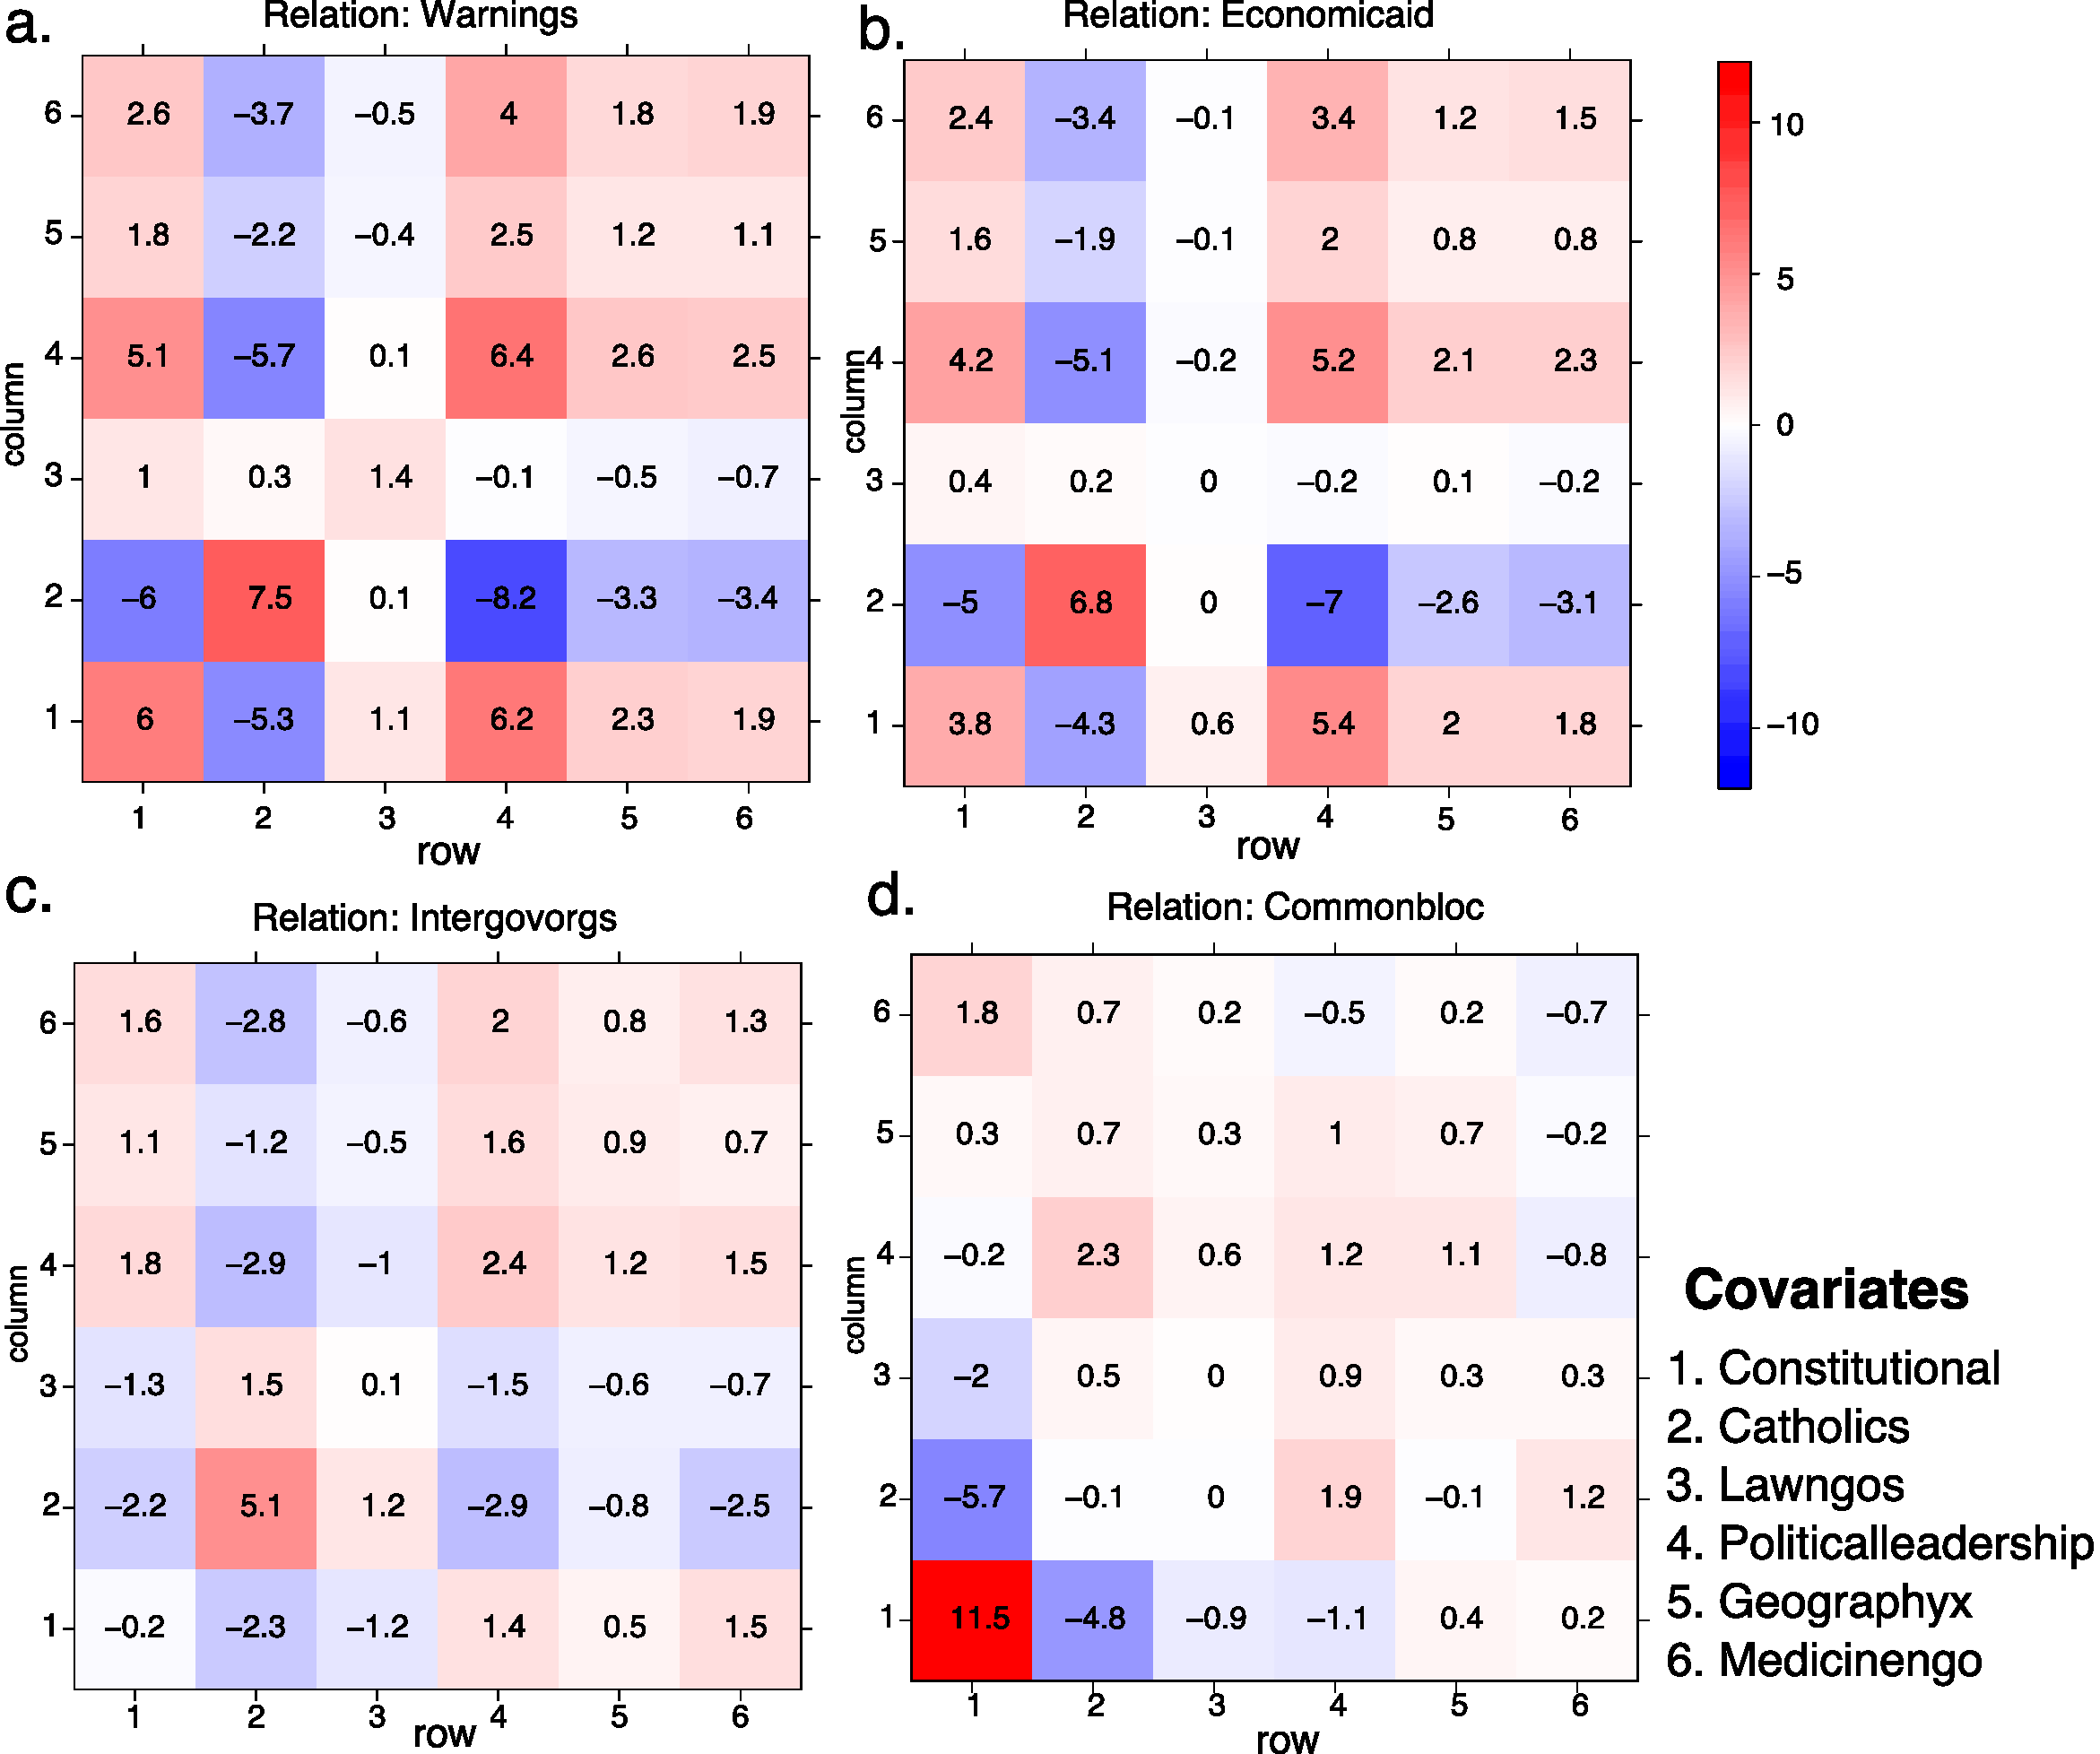
\includegraphics[width=8cm]{coef.pdf}
\caption{Effect estimation in the \emph{Nations} data. Panels (a)-(d) represent the estimated effects of country-level attributes towards the connection probability, for relations \emph{warnning}, \emph{economicaid},\emph{intergovorg}, and \emph{commonblock}, respectively. }\label{fig:est}
\end{figure}
Supplement table~\ref{tab:s1} summarizes the $K$-means clustering of the 56 relations based on the $3^{\text{rd}}$ mode factor $\mM_3\in\mathbb{R}^{56\times 4}$ in the tensor regression model. 

\begin{table}[ht]
\begin{tabular}{c|l}
\hline
\multirow{4}{*}{Cluster I}  &officialvisits, intergovorgs,  militaryactions, violentactions, duration, \\
&negativebehavior, boycottembargo, aidenemy, negativecomm, accusation, \\
& protestsunoffialacts,    nonviolentbehavior, emigrants, relexports,   \\
& timesincewar, commonbloc2, rintergovorgs3, relintergovorgs\\
\hline
\multirow{4}{*}{Cluster II}& economicaid, booktranslations, tourism, relbooktranslations, releconomicaid, \\
& conferences, severdiplomatic, expeldiplomats, attackembassy, unweightedunvote,\\
& reltourism, tourism3, relemigrants, emigrants3, students, relstudents, \\
&exports, exports3, lostterritory, dependent, militaryalliance, warning  \\
\hline
\multirow{2}{*}{Cluster III} & treaties, reltreaties, exportbooks, relexportbooks, weightedunvote, ngo, \\
&relngo, ngoorgs3, embassy, reldiplomacy, timesinceally, independence, commonbloc1\\
\hline
Cluster IV & commonbloc0, blockpositionindex\\
\hline
\end{tabular}
\caption{$K$-means clustering of relations based on factor matrix in the coefficient tensor.}\label{tab:s1}
\end{table}

\clearpage
\bibliographystyle{unsrt}
\bibliography{tensor_wang}

\end{document}